
% !TEX encoding = UTF-8 Unicode
% -*- coding: UTF-8; -*-
\ifdefined\ishandout
\documentclass[handout]{beamer}
\else
\documentclass[11pt]{beamer}
\fi

\usepackage[frenchb]{babel}
\usepackage[T1]{fontenc}
\usepackage[utf8]{inputenc}
\usepackage{hyperref}
\usepackage{multirow}
\usepackage{listings}
\usepackage{fancyvrb}
\usepackage{tikz}
\usepackage{framed}
\usepackage{algorithm}
\usepackage{algorithmic}
\usepackage{xcolor}
\usepackage{color, colortbl}
\ifdefined\ishandout
\usepackage{handoutWithNotes}
\fi
\usepackage{slashbox}
\usepackage{amsmath}
\usepackage{bm}
\usepackage{hhline}
\usepackage{xmpmulti}

\usetikzlibrary{shapes.geometric}
\usetikzlibrary{positioning}
\usetikzlibrary{shapes.arrows, chains}
\usetikzlibrary{arrows,calc}
\usetikzlibrary{shapes.multipart}
\usepackage{array}
\usetheme{Boadilla}

\usefonttheme[onlymath]{serif}

\newcommand{\R}{\mathbb{R}}
\newcommand{\C}{\mathbb{C}}
\newcommand{\N}{\mathbb{N}}
\newcommand{\Z}{\mathbb{Z}}
\newcommand{\E}{\mathbb{E}}
\newcommand{\Var}{\text{Var}}
\newcommand{\Cov}{\text{Cov}}
\ifdefined\ishandout
\pgfpagesuselayout{3 on 1 with notes}[a4paper,border shrink=5mm]
\usecolortheme{dove}
\else
%\usecolortheme{dolphin}
\usecolortheme{beaver}
\fi


\lstnewenvironment{codeC}
{ \lstset{language=C,
    otherkeywords={printf,scanf}}
}
{}

\ifdefined\ishandout
\definecolor{mygreen}{rgb}{0,0,0}
\definecolor{mymauve}{rgb}{0,0,0}
\definecolor{myblue}{rgb}{0,0,0}
\else
\definecolor{mygreen}{rgb}{0,0.6,0}
\definecolor{mymauve}{rgb}{0.58,0,0.82}
\definecolor{myblue}{rgb}{0,0,1}

\fi

%% Notes
%\setbeameroption{show only notes}


\definecolor{mygray}{rgb}{0.5,0.5,0.5}

\lstset{ language=Python,%
  backgroundcolor=\color{white},   % choose the background color; you must add \usepackage{color} or \usepackage{xcolor}
  basicstyle=\footnotesize,        % the size of the fonts that are used for the code
  breakatwhitespace=false,         % sets if automatic breaks should only happen at whitespace
  breaklines=true,                 % sets automatic line breaking
  captionpos=b,                    % sets the caption-position to bottom
  commentstyle=\color{mygreen},    % comment style
  deletekeywords={...},            % if you want to delete keywords from the given language
  escapeinside={\%*}{*)},          % if you want to add LaTeX within your code
  extendedchars=true,              % lets you use non-ASCII characters; for 8-bits encodings only, does not work with UTF-8
  frame=tb,	                   % adds a frame around the code
  keepspaces=true,                 % keeps spaces in text, useful for keeping indentation of code (possibly needs columns=flexible)
  keywordstyle=\color{blue},       % keyword style
  otherkeywords={*,...},           % if you want to add more keywords to the set
  numbers=none,                    % where to put the line-numbers; possible values are (none, left, right)
  numbersep=5pt,                   % how far the line-numbers are from the code
  numberstyle=\tiny\color{mygray}, % the style that is used for the line-numbers
  rulecolor=\color{black},         % if not set, the frame-color may be changed on line-breaks within not-black text (e.g. comments (green here))
  showspaces=false,                % show spaces everywhere adding particular underscores; it overrides 'showstringspaces'
  showstringspaces=false,          % underline spaces within strings only
  showtabs=false,                  % show tabs within strings adding particular underscores
  stepnumber=2,                    % the step between two line-numbers. If it's 1, each line will be numbered
  stringstyle=\color{mymauve},     % string literal style
  tabsize=3,	                   % sets default tabsize to 2 spaces
  title=\lstname                   % show the filename of files included with \lstinputlisting; also try caption instead of title
}
%\lstset{language=Python,
% breakatwhitespace=false,         % sets if automatic breaks should only happen at whitespace
%  breaklines=true,                 % sets automatic line breaking
%  captionpos=b,                
%%commentstyle=\itshape\color{mymauve},
%%keywordstyle=\bfseries\color{myblue},
%numbers=left,                    % where to put the line-numbers; possible values are (none, left, right)
%  numbersep=8pt,                   % how far the line-numbers are from the code
%  numberstyle=\tiny\color{mygray}, % the style that is used for the line-numbers
%%  rulecolor=\color{black},         % if not set, the frame-color may be changed on line-breaks within not-black text (e.g. comments (green here))
%  showspaces=false,                % show spaces everywhere adding particular underscores; it overrides 'showstringspaces'
%%  showstringspaces=false,          % underline spaces within strings only
%  showtabs=false,                  % show tabs within strings adding particular underscores
%  stepnumber=2,                    % the step between two line-numbers. If it's 1, each line will be numbered
%%  stringstyle=\color{mygreen},     % string literal style
%  tabsize=2 
%}
\ifdefined\ishandout
\newcommand{\red}{\textbf}
\else
\newcommand{\red}{\textcolor{red}}
\fi
%\newcommand \emph
%Default size : 12.8 cm * 9.6 cm

\newcommand{\tmark}[1]{\tikz[remember picture, baseline=-.5ex]{\coordinate(#1);}}

\ifdefined\ishandout
\newenvironment<>{codeblock}[1]{%begin
  \setbeamercolor{block title}{fg=black,bg=lightgray!80}%
  \begin{block}{#1}}
  % \begin{codeC}}
  %  {\end{codeC}
{  
\end{block}}

\newenvironment<>{termblock}[1]{
    \setbeamercolor{block title}{fg=black,bg=lightgray!90}%
    \begin{block}{#1}
}
%     \begin{Verbatim}}
{%\end{Verbatim}
\end{block}
}

\definecolor{bluegreen}{RGB}{0,0,0}
%\definecolor{bluegreen}{rgb}{0,0.6,0.8}
\else

\newenvironment<>{codeblock}[1]{%begin
  \setbeamercolor{block title}{fg=darkgray,bg=yellow}%
  \begin{block}{#1}}
  % \begin{codeC}}
  %  {\end{codeC}
{  
\end{block}}

\newenvironment<>{termblock}[1]{
    \setbeamercolor{block title}{fg=white,bg=lightgray}%
    \begin{block}{#1}}
%     \begin{Verbatim}}
{%\end{Verbatim}
\end{block}
}

\definecolor{bluegreen}{RGB}{0,149,182}
%\definecolor{bluegreen}{rgb}{0,0.6,0.8}
\fi

%\newcommand{\output}[1]{
\setbeamertemplate{navigation symbols}{}
\newcommand{\bvrb}{\Verb[commandchars=£µ§,formatcom=\color{bluegreen}]}
\newcommand{\footvrb}{\footnotesize\Verb}
\newcommand{\vrbalert}[2][]{\visible<#1>{#2}}
%%% Commande pour les listes/arbres
\newcommand{\mvide}{\nodepart{one} \nodepart{two}}
\newcommand{\tvide}{\nodepart{one} \nodepart{two} \nodepart{three}}
\newcommand{\rref}[1][]{\hfill{\scriptsize\textit{#1}}}


\newcommand{\odif}[2]{\frac{d #1}{d #2}} 
%%Fin des commandes pour les listes/arbres.
\newcommand{\gooditem}[1]{\setbeamercolor{item}{fg=green}\item #1} 
\newcommand{\pooritem}[1]{\setbeamercolor{item}{fg=red}\item #1} 
\setbeamerfont{caption}{size=\scriptsize}

%%% Paramètres du cours (à régler)
%Numéro du cours
\newcommand{\nb}{1}

\title[lagrangian assimilation]{Assimilation of non-conventional observations. Application to the estimating of ocean surface currents.}
\author[J. Brajard]{julien.brajard@upmc.fr}
\institute[LOCEAN/UPMC]{LOCEAN-UPMC}
\date{8 june 2017}
\begin{document}
\tikzstyle{every picture}+=[remember picture]
%%%%%%%%%%%%%%%%%%%%% SLIDES DE TITRE
\begin{frame}
\titlepage
%\centering{
%\url{http://australe.upmc.fr} (onglet EPU-C5-IGE Info Gen)}
\end{frame}

%%%%%%%%%%%%%%%%%%%%
\begin{frame}
\frametitle{LOCEAN institute}
\begin{figure}

\includegraphics[height=0.1\textheight]{../../fig/logo-locean.png}
\end{figure}
Laboratory in University Pierre et Marie Curie with scientific thematics :
\begin{itemize}
\item Physical oceanography
\item Marine bio-geochemistry
\item Climate
\item Paleocenography
\item ...
\end{itemize}
Using a wide spectra of approaches:
\begin{itemize}
\item Numerical modelling
\item Statistical modelling
\item Observations (campaigns, or autonomous plateforms)
\item Remote-sensing
\end{itemize}
\end{frame}
%%%%%%%%%%%%%%%%%%%%%
\begin{frame}
\frametitle{Data assimilation}
\begin{block}{Objective}
Optimally combine output of an numerical model and some observations
\end{block}
\begin{tikzpicture}
\draw[thick,->](-0.2,0)--(10,0) node[below]{$time$};
\draw[thick,->](0,-0.2)--(0,5) node[left]{$x$};
\draw[red,very thick] plot [smooth] 
coordinates {(0,1)  (1,1)  (3,2) (5,0.5) (7,4) (9,3) } ;
\draw plot [mark=*, mark size=5pt, only marks, mark options={color=red}]
coordinates{(0,1)} node [left,xshift=-0.5em]{\textcolor{red}{$x^b$}};
\draw <2-> plot [mark=*, mark size=3pt, only marks, mark options={color=blue}]
coordinates {(0.5,2) (3,3) (4,0.5) (6,4.5) (8,3)};
\draw <3-> [magenta,very thick] plot [smooth] 
coordinates {(0,2)  (1,2.5)  (3,2.8) (4.6,0.1) (6,4) (9,2.5) } ;
\draw <3-> plot [mark=*, mark size=5pt, only marks, mark options={color=magenta}]
coordinates{(0,2)} node [left,xshift=-0.5em]{\textcolor{magenta}{$x^a$}};
\draw (0.1,5.4) node [anchor=west] {\textcolor{red} {$-$ background}};
\draw <2-> (0.1,4.8) node [anchor=west] {\textcolor{blue} {$\bullet$ observations}};
\draw <3-> (0.1,4.2) node[anchor=west]  {\textcolor{magenta} {$-$ analyze}};
\end{tikzpicture}
\end{frame}


%%%%%%%%%%%%%%%%%%%%%%
\begin{frame}
\frametitle{Some equations...}
The basics ingredients for data assimilation are :
\begin{itemize}[<+->]
\item A state vector: $\bm{x_k}$
\item A dynamical model (with error): $\bm{x_k} = M_k(\bm{x_{k-1}}) +
  \bm{w_k}$
\item Some observations at time $\bm{k}$: $\bm{y_k} = H_k(\bm{x_k}) +
  \bm{v_k}$
\item An background state (often at time 0): $\bm{x^b_0} = \bm{x_0} +
  \bm{e}$
\item Error statistics: 
\begin{itemize}
\item $\E[\bm{w_kw_k^T}] = \bm{Q_k}$
\item $\E[\bm{v_kv_k^T}] = \bm{R_k}$
\item $\E[\bm{ee^T}] = \bm{B}$
\end{itemize}
\end{itemize}
\pause
\begin{alertblock}{Objective}
Estimate the more likely state $\bm{x_k^a}$ knowing
$M$,$H$,$\bm{y}$,$\bm{x^b}$,$\bm{Q}$,$\bm{R}$ and $\bm{B}$
\end{alertblock}
\end{frame}

%%%%%%%%%%%%%%%%%%%%%%%%%%%
\begin{frame}
\frametitle{Minimization problem}
\tikzstyle{na} = [baseline=-.5ex]
\begin{block}{Cost function}
Finding the best estimate $\bm{x^a}=\left(\bm{x_0^a} \cdots \bm{x_k^a}\cdots\bm{x_n^a} \right)$ is equivalent to find the value minimizing $\mathcal{J}(\bm{x_0})$
\end{block}
\begin{itemize}
\item Error on the observations \tikz[na] \node [coordinate] (n1) {};
\end{itemize}
\begin{align}
\mathcal{J}(\bm{x_0}) & =  
\tikz[baseline]{ \node[fill=blue!20,anchor=base] (t1)
{$\sum _{k=0}^{K} 
  \left(\bm{y_k} -  \bm{H_k}\bm{x_k}\right)^T
  \bm{R_k}^{-1}
  \left(\bm{y_k} -  \bm{H_k}\bm{x_k}\right)
 $};
}
\nonumber \\
& + \tikz[baseline]{ \node[fill=red!20,anchor=base] (t2)
{$\frac{1}{2} \left(\bm{x_0}-\bm{x_0^b}\right)^T\bm{B_0}^{-1} \left(\bm{x_0}-\bm{x_0^b}\right)$};}
\end{align}
\begin{itemize}
\item  Error on the background \tikz[na] \node
  [coordinate] (n2) {};
\item Model is supposed to be "perfect" (no model error):$\bm{x_k} = \bm{M_k}\bm{x_{k-1}}$
\end{itemize}
\begin{tikzpicture}[overlay]
        \path[->] (n1) edge [bend left] (t1);
        \path[->] (n2) edge [bend right] (t2);
\end{tikzpicture}
\end{frame}


%%%%%%%%%%%%%%%%%%%%%%%%%%%
\begin{frame}
\frametitle{A solution ?}
\begin{block}{Analytic solution}
The solution of Eq.1 is:
$$ \bm{x_0^a} = \bm{x_0^b} - \mathcal{H}^{-1}\nabla_{\bm{x_0}}\mathcal{J}(\bm{x_0^b})
$$
where $ \mathcal{H} = \bm{B}^{-1} + \sum_{k=0}^n \bm{M_{k,0}}^T\bm{H_k}^T\bm{R_k}^{-1}\bm{H_k}\bm{M_{k,0}}$
\end{block}
\begin{alertblock}{Impossible to compute if:}
\begin{itemize}
\item The size of $\bm{x_k}$ is too big (typically $\approx 10^5$)
\item $\bm{H_k}$ and/or $\bm{M_{k,0}}$ are non-linear 
\end{itemize}
\end{alertblock}
\end{frame}

%%%%%%%%%%%%%%%%%%%%%%%%%%%
\begin{frame}
\frametitle{Gradient descent technique}

\begin{figure}
\centering
\begin{tikzpicture}[
auto,
>=stealth',
box/.style={rectangle, draw, fill=blue!20}]
\node (x0) {$\bm{x_0}$};
\node [box,minimum width=7em,minimum height=2em] (M) [right=of x0]{\alt<2>{\red{Direct model}}{$\bm{M_{k,0}}$}} edge [<-] (x0);
\node (xk) [right=of M]{$\bm{x_k}$} edge [<-] (M);
\node [box] (J) [right=of xk]{$\mathcal{J}$} edge [<-] (xk);
\node (y) [above=of J]{$\bm{y_k}$} edge [->] (J);
\node (Jx0) [right=of J]{$\mathcal{J}(\bm{x_0})$} edge [<-] (J);
\node [box] (adjy) [below=of J]{$ \nabla_{\bm{y}}\mathcal{J}$};
\path [->,draw] (Jx0) |- (adjy);
\node (dy) [left=of adjy] {$\Delta$} edge [<-] (adjy);
\node [box,minimum width=7em,minimum height=2em] (adj) [left=of dy]{\alt<2>{\red{Adjoint model}}{$\bm{M_{k,0}}^T$}} edge [<-] (dy) ; 
\node (dx) [left=of adj] {$\Delta_x$} edge [<-] (adj);
\path[->,draw] (dx) edge [bend left] (x0);

\end{tikzpicture}
\end{figure}

\begin{block}{Gradient}
$$ \nabla_{\bm{x_0}}\mathcal{J} = \bm{B}^{-1}\left(\bm{x_0}-\bm{x_0^b}\right) - 
\sum_{k=0}^n\bm{M_{k,0}}^T \Delta_y $$
with $\Delta_y = \bm{H_k}^T \bm{R_k}^{-1} \left(\bm{y_k}-\bm{H_k}\bm{M_{k,0}}\bm{x_0}\right) $
\end{block}
\end{frame}


%%%%%%%%%%%%%%%%%%%%%%%%%%
\begin{frame}
\frametitle{Implementation issues}
\begin{columns}[t]
\column{.48\textwidth}
\begin{block}{Traditionnal approach}
\begin{enumerate}
\item Code for the direct model
\item Code for the adjoint model
\item Code for the assimilation scheme
\end{enumerate}
\end{block}
\begin{itemize}
\gooditem Fine tuning of the optimization
\pooritem Difficult to maintain
\pooritem Validation of the correspondance between direct/adjoint
model is difficult.
\end{itemize}
\column{.48\textwidth}
\begin{block}{Automatic approach}
\begin{tikzpicture}[auto,
node distance = 0.5cm,
>=stealth',
box/.style={text badly centered,rectangle, text width=.9\textwidth,draw,fill=red!20},
txt/.style={text badly centered,text width=.9\textwidth}]
\node [txt] (n1)  {Description of the model using a modular graph};
\node [box] (n2) [below = of n1] {YAO code generator} edge [<-] (n1);
\node [txt] (n3) [below = of n2] {\vbox{
\begin{itemize}
\item Direct model
\item Adjoint model
\item toolbox for assimilation/validation
\end{itemize}}} edge [<-] (n2);
\end{tikzpicture}
\end{block}
\end{columns}
\end{frame}

%%%%%%%%%%%%%%%%%%%%%%%%%
\begin{frame}
\frametitle{Validation of the adjoint code}
\begin{block}{How to check if the adjoint is correct}
$$
R(\alpha) = J(x=\alpha dx) - J(x) - \alpha dx . \nabla_x J(x) =
o(\alpha^2)
$$
\end{block}
\begin{figure}
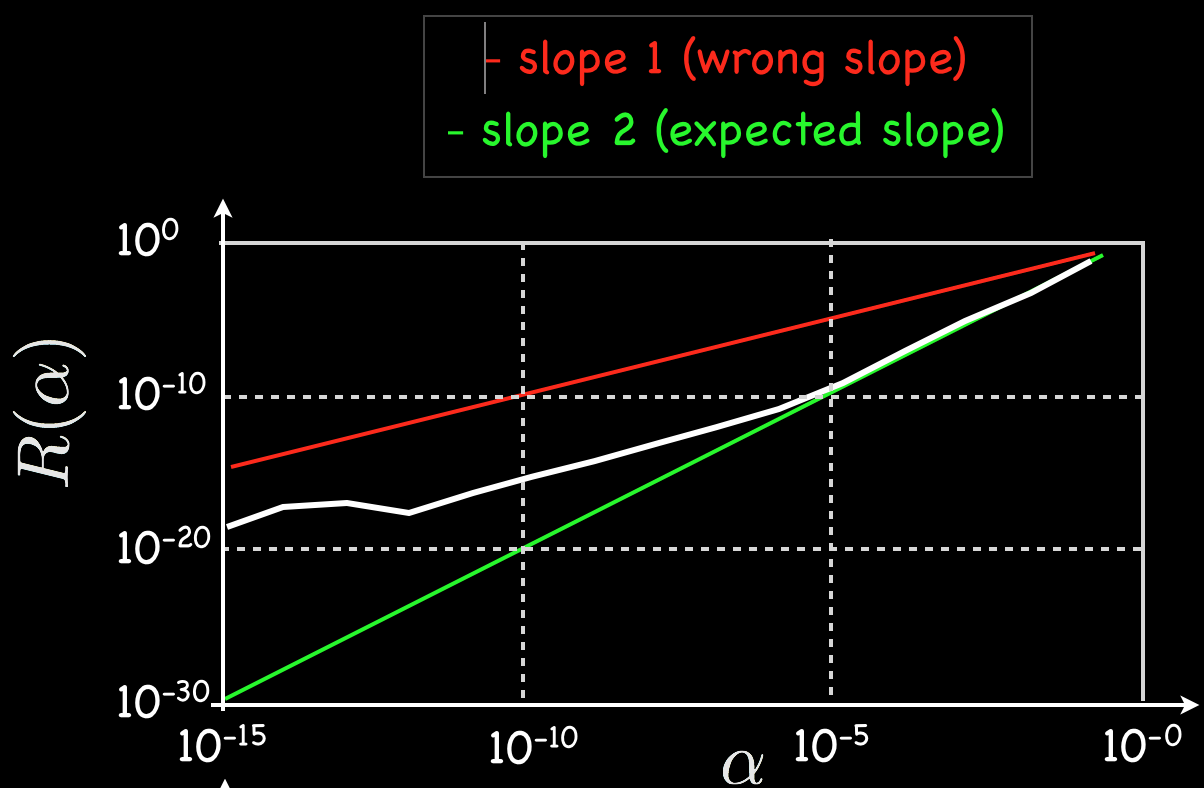
\includegraphics[width=.7\textwidth]{./fig/adj-ieee.png}
\end{figure}

\end{frame}

%%%%%%%%%%%%%%%%%%%%%%%%%%%%
\begin{frame}
\frametitle{Numerical validation}
\begin{block}{Why is the test incorrect ?}
\begin{itemize}
\item Effective error in the adjoint code
\item Inaccuracy due to round-off errors
\end{itemize}
\end{block}
\begin{alertblock}{A solution}
CADNA
\end{alertblock}
\end{frame}

%%%%%%%%%%%%%%%%%%%%%%%%%%%%%
\begin{frame}
\frametitle{Result}
\begin{columns}
\column{.5\textwidth}
\begin{figure}
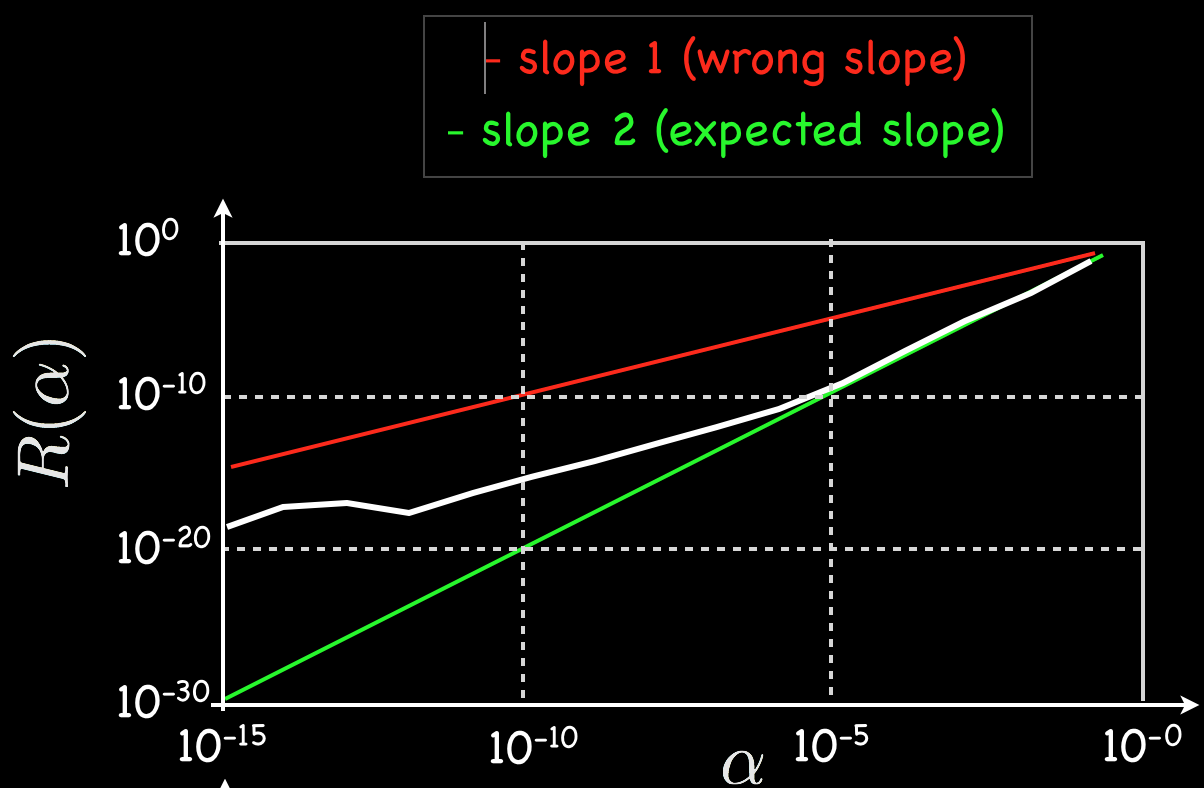
\includegraphics[width=.9\textwidth]{./fig/adj-ieee.png}
\caption{Without CADNA}
\end{figure}
\column{.5\textwidth}
\begin{figure}
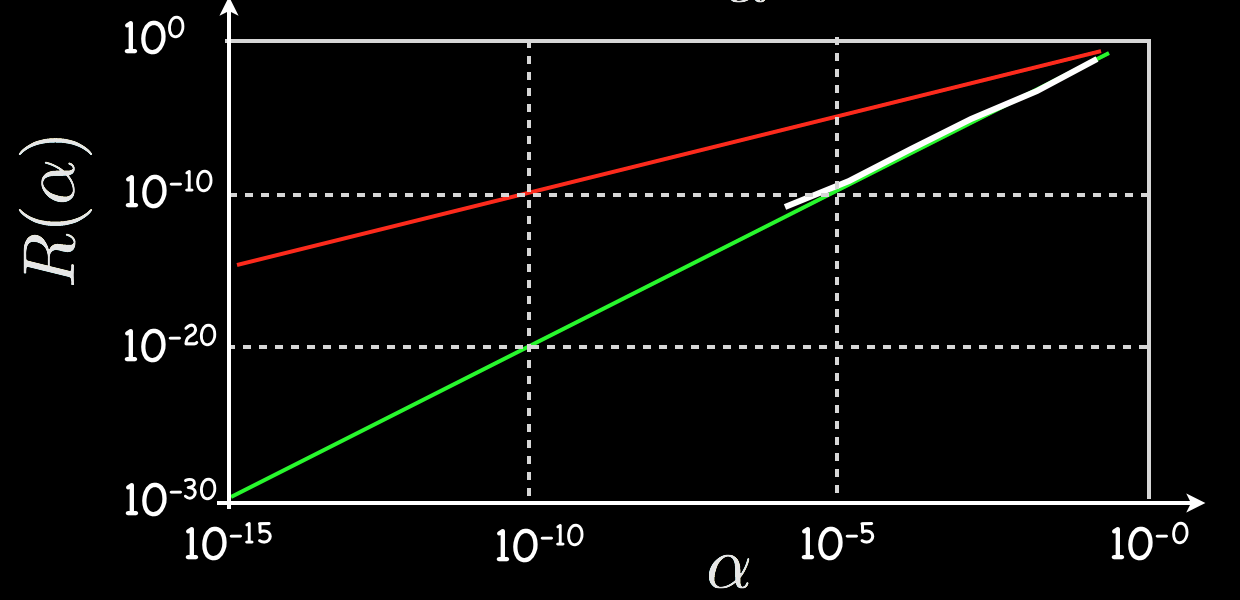
\includegraphics[width=.9\textwidth]{./fig/adj-cadna.png}
\caption{With CADNA}
\end{figure}
\end{columns}
\end{frame}

%%%%%%%%%%%%%%%%%%%%%%%%%%%
\begin{frame}
\frametitle{Example of the sallow-water problem}
\begin{block}{Shallow-water equations}
Shallow-water equations (derived from Navier and Sockes) describe the
flow of a fluid (e.g. the water) homogenous in the vertical.
\end{block}
\begin{columns}
\column{.5\textwidth}
\begin{figure}
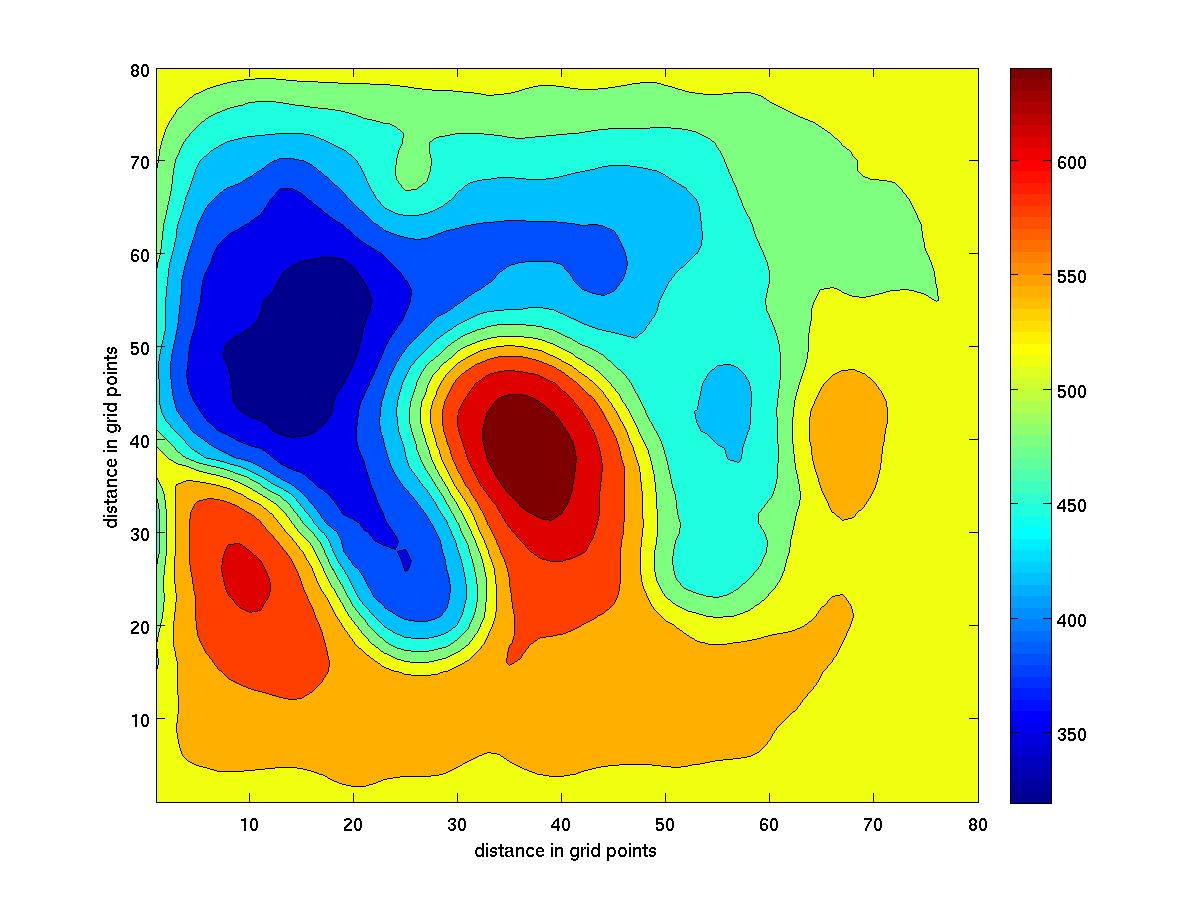
\includegraphics[width=.9\textwidth]{./fig/xt_fin.jpg}
\caption{Water height at t=0}
\end{figure}
\column{.5\textwidth}
\begin{itemize}
\item Size of the simulation window : 3 months
\item Spin-up: 10 years
\end{itemize}
\end{columns}


\end{frame}
%%%%%%%%%%%%%%%%%%%%%%%%%%%
\begin{frame}
\frametitle{Assimilation data setup}
\begin{itemize}
\item Twin experiment using the reference simulation
\item Ensemble experiment (30 assimilations to evaluate the uncertainty)
\item Assimilation window : 3 months
\item Control parameter : $h_0$
\item Observations : 
\begin{itemize}
\item 30 000 observations 
\item randomly sampled on the whole assimilation window 
\item perturbed by a white gaussian noise ($\sigma=1m$).
\end{itemize}
\item Background: white gaussian noise ($\sigma=10m$).
\end{itemize}
\vspace{-1em}
\end{frame}

%%%%%%%%%%%%%%%%%%%%%%%%%%%%%%
\begin{frame}
\frametitle{Cost function minimization}
\framesubtitle{Temps de l'expérience sur un PC : 3h}

\begin{figure}
\centering
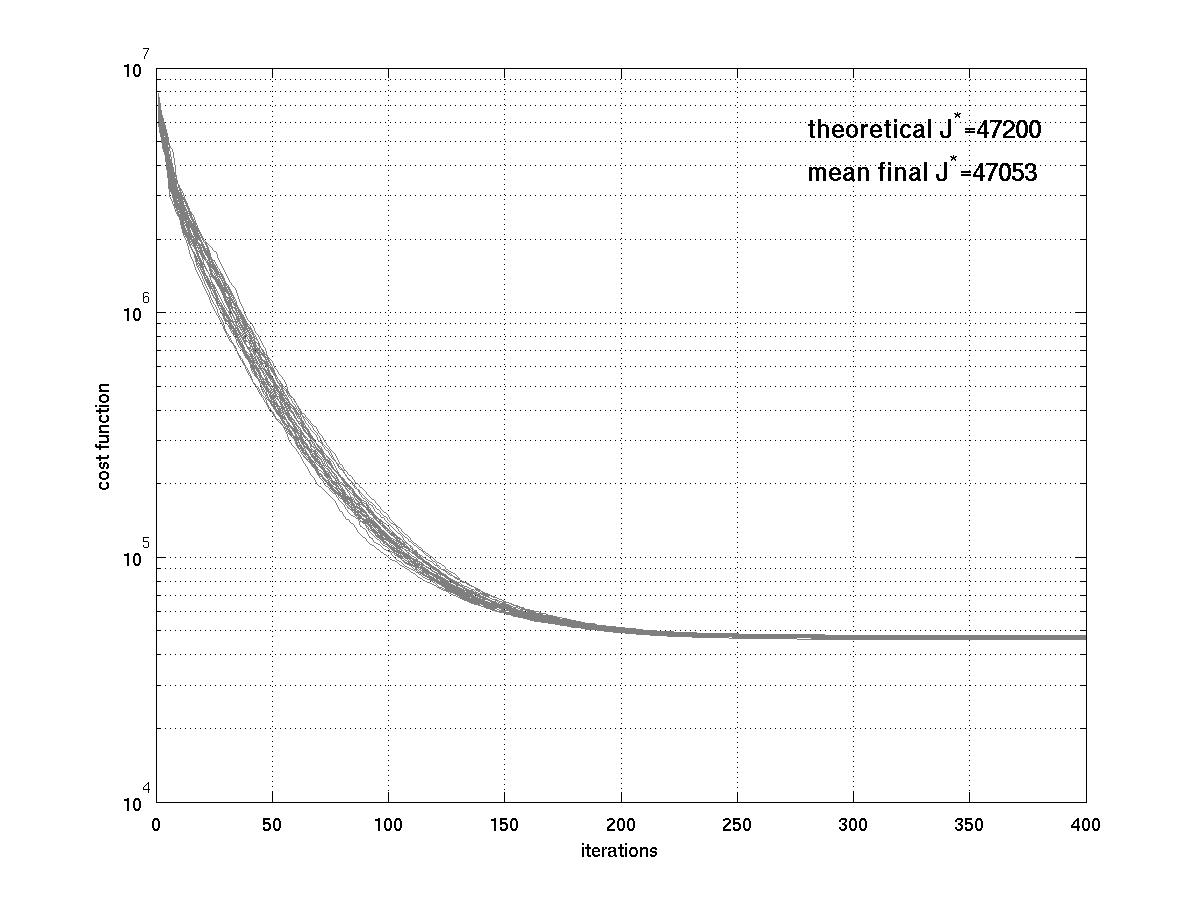
\includegraphics[width=.8\textwidth]{./fig/cost.jpg}\\
\caption{Minimisation of the cost function $\mathcal{J}$}
\end{figure}

{\footnotesize $30000-6400 = 23600 = J_{min}/2$}
%% Plot of all cost functions
%% histogram
\end{frame}

\begin{frame}
\frametitle{Preliminary results}
\begin{columns}[t]

\column{.3\textwidth}
\begin{figure}
\centering
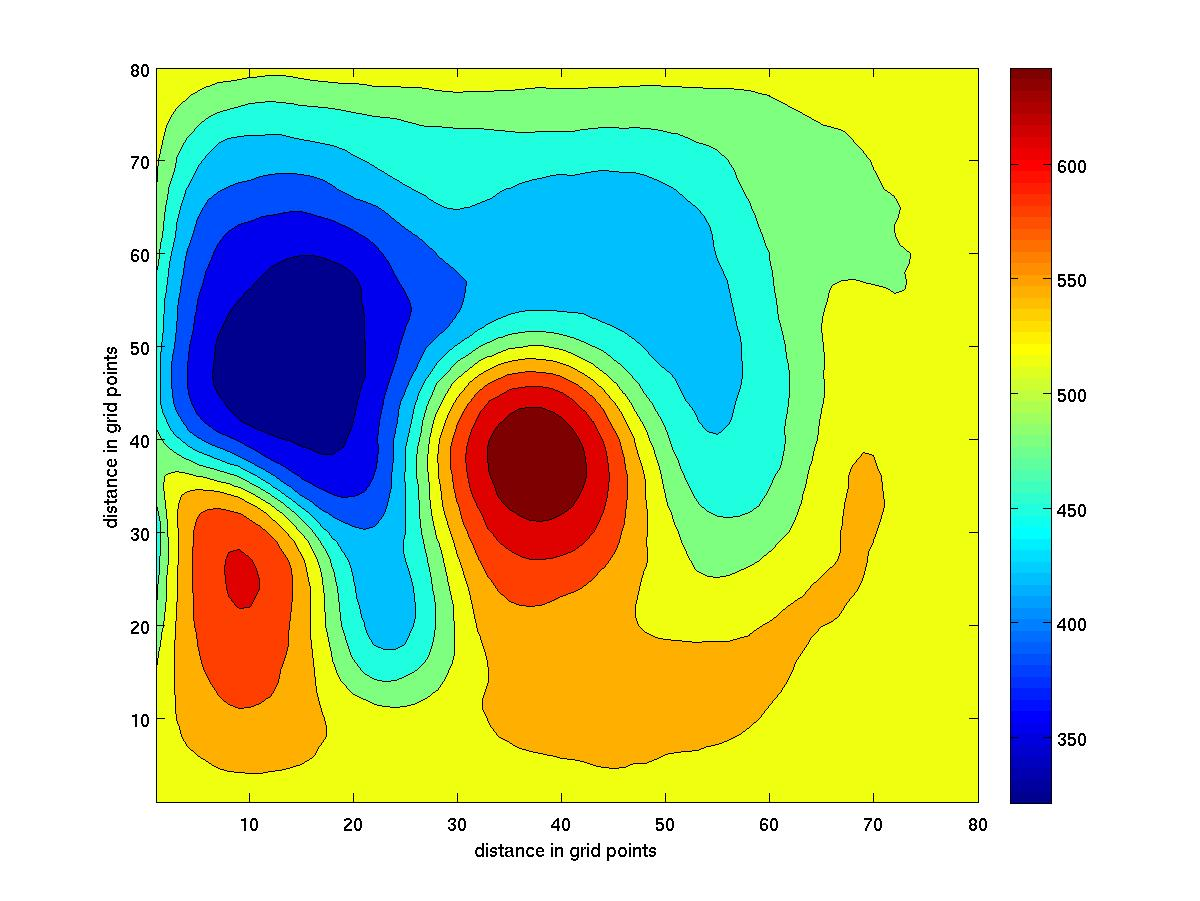
\includegraphics[width=4.2cm]{./fig/xb_fin.jpg}\\
\caption{Background field at t=1 month}
\end{figure}

\column{.3\textwidth}
\begin{figure}
\centering
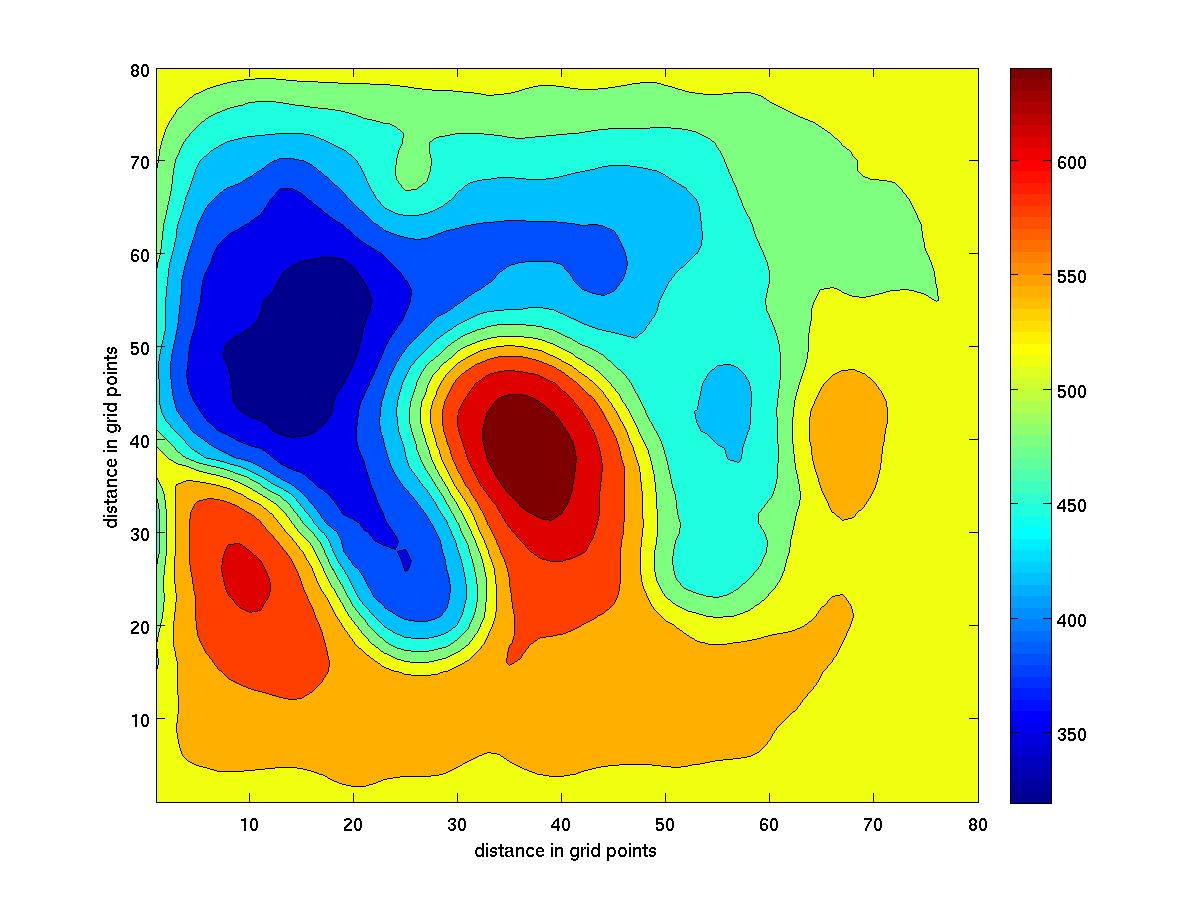
\includegraphics[width=4.2cm]{./fig/xt_fin.jpg}\\
\caption{True field at t=1month}

\end{figure}


\column{.3\textwidth}
\begin{figure}
\centering
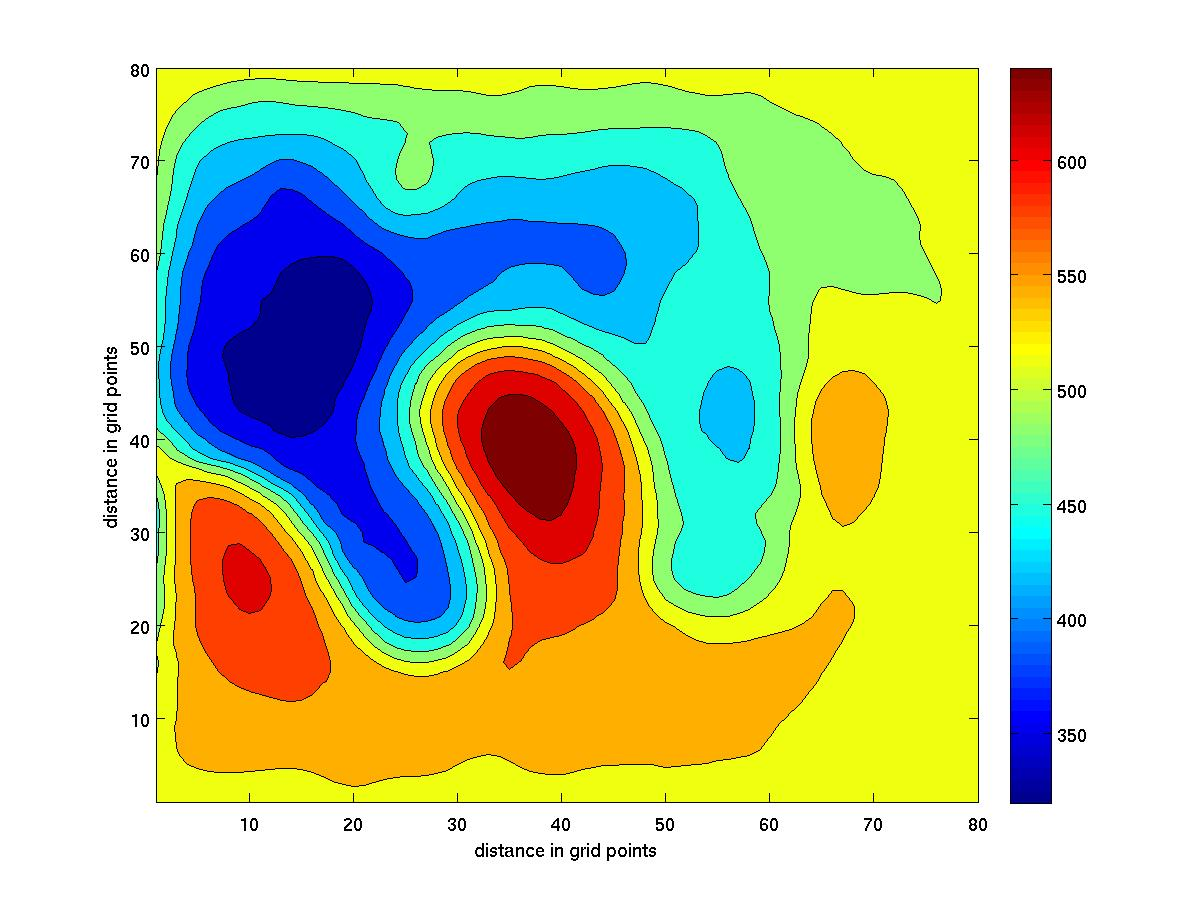
\includegraphics[width=4.2cm]{./fig/xa_fin.jpg}\\
\caption{Analysed height field at t=1 month}

\end{figure}


\end{columns}

\vspace{2em}

\end{frame}

\begin{frame}
\frametitle{Errors}

\begin{columns}[t]

\column{.45\textwidth}
\begin{figure}
\centering
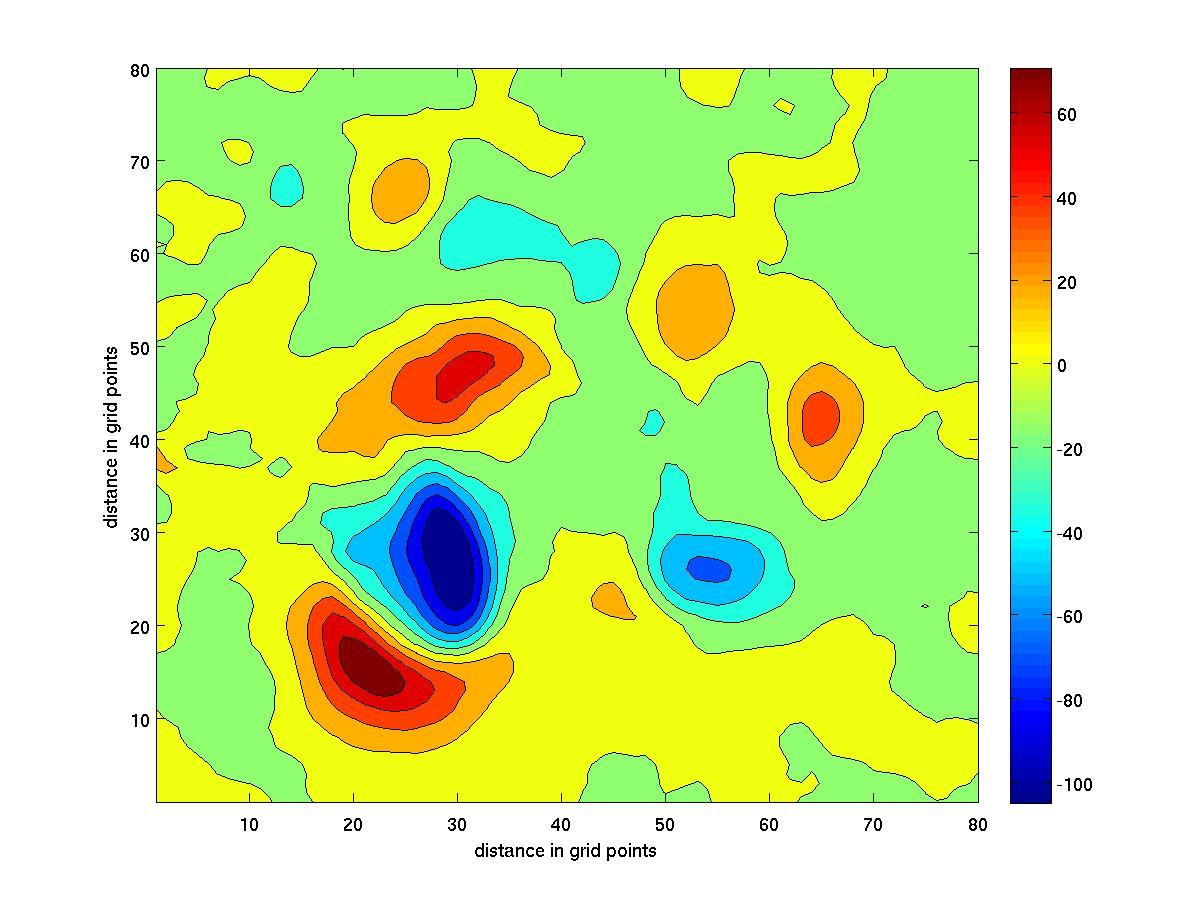
\includegraphics[width=6cm]{./fig/diff_bt.jpg}\\
\caption{Error at t=3 month between backround and "truth"}
\end{figure}
\column{.45\textwidth}
\begin{figure}
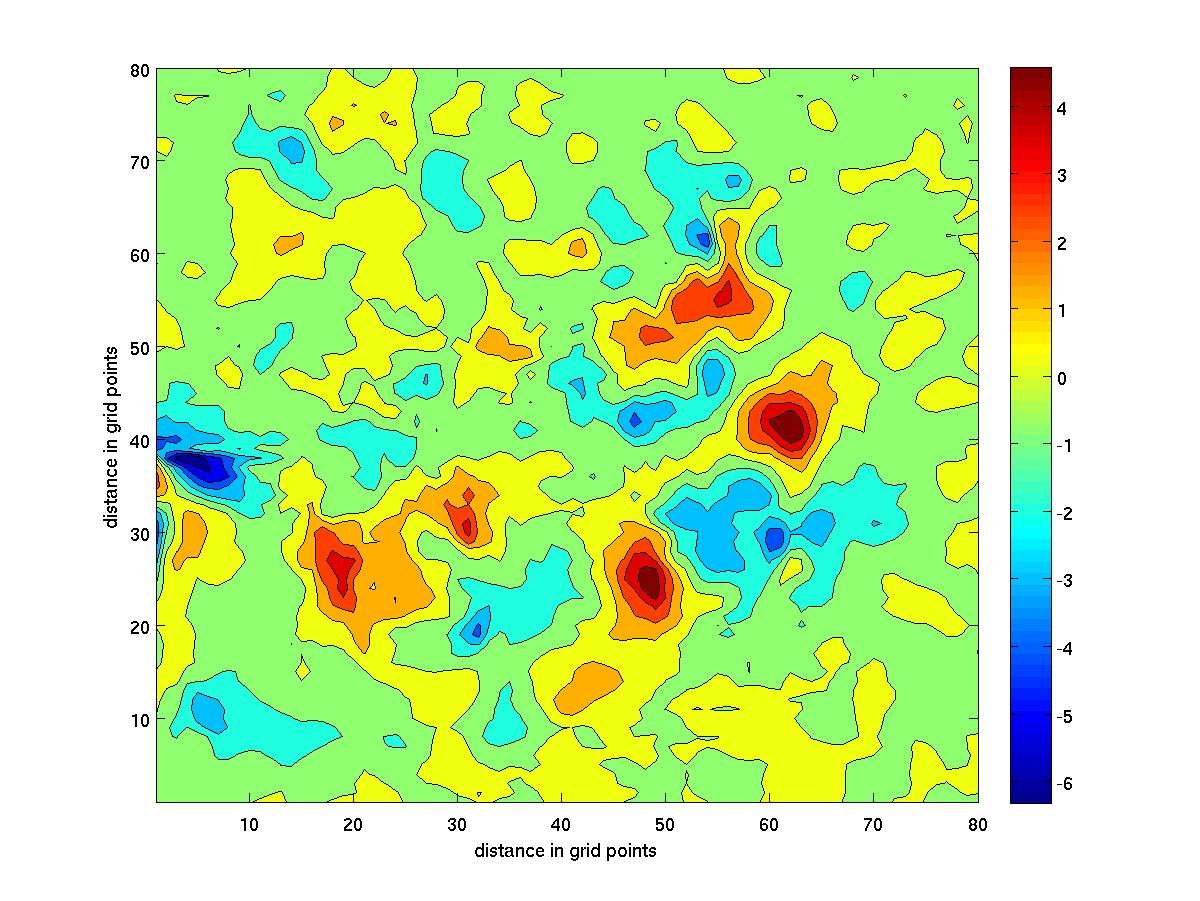
\includegraphics[width=6cm]{./fig/diff_at.jpg}\\
 \caption{Error at t=3 months between analysis and "truth"}
\end{figure}
\end{columns}
\end{frame}

\begin{frame}[t]
\frametitle{Solution in time}
\framesubtitle{Water height at point x=45 et y=60}
\begin{figure}
\centering
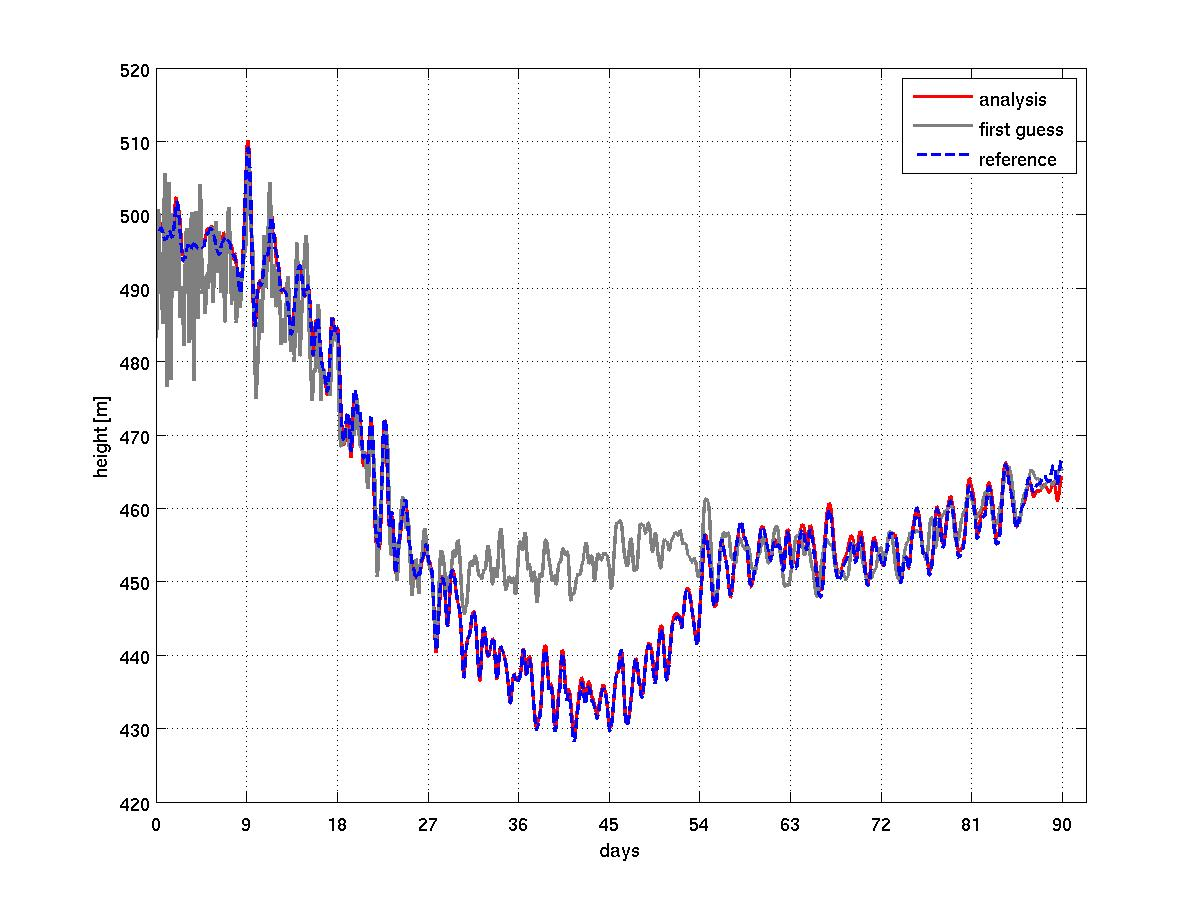
\includegraphics[width=10.5cm]{./fig/trajectory.jpg}\\
\end{figure}
\end{frame} 


%%%%%%%%%%%%%%%%%%%%%%%%%%%
\begin{frame}
\frametitle{Conclusion}
Data assimilation is an efficient and operational method to combine a
numerical model and observations. It involves several scientific
themes in link with LIP6:
\begin{itemize}
\item Optimization
\item Computation using large datasets
\item Numerical validation
\item High Performance Computing
\end{itemize}
\end{frame}

\end{document}